\chapter{Architectuur van het ontworpen systeem}\label{hs:architectuur}

In dit hoofdstuk wordt de architectuur van het systeem beschreven zonder concreet in
te gaan op de implementatie. Het doel is om de ontwerpkeuzes te verdedigen. Details in verband met de werking komen in hoofdstuk \ref{hs:werking}. 

\section{Algemeen overzicht}

Figuur \ref{fig:overzicht-architectuur} geeft een high-level overzicht van de architectuur van het volledige systeem. Alle onderdelen van het ontworpen systeem zijn onderling onafhankelijk van elkaar. Dit maakt een robuuste, gedistribueerde eenheid waaraan relatief eenvoudig nieuwe componenten kunnen worden toegevoegd. Elk onderdeel wordt in de volgende paragrafen besproken.

\begin{figure}[h]
	\caption{High-level overzicht van de architectuur}
	\label{fig:overzicht-architectuur}
	
	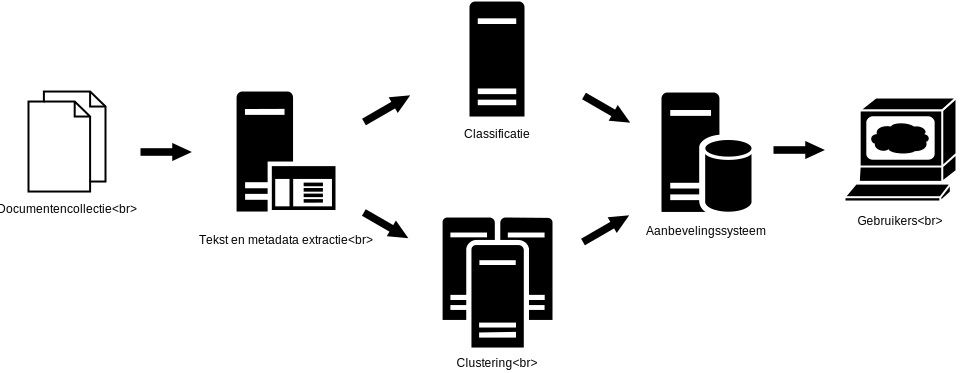
\includegraphics[width=\textwidth]{fig/thesis-overview.png}
\end{figure}

\subsection{Tekst en metadata extractie}
Tekstuele data kan verschijnen onder verschillende vormen: HTML-pagina's, pdf-documenten, Word-documenten, etc. Elk van deze vormen heeft zijn eigen vorm en opmaak om de representatie als het ware up te graden van platte tekst naar iets wat bruikbaar is binnen hun eigen omgeving. Zo worden bij HTML verschillende tags toegevoegd om de opmaak te verfraaien of wordt er bij pdf-documenten een fixed-layout gemaakt om het document er onder alle omstandigheden hetzelfde te laten uitzien. 

Om met deze verschillende soorten van tekst te kunnen werken binnen een systeem van content recognition is het belangrijk om de platte tekst uit deze verschillende documentenformaten te extraheren. Op die manier wordt een gemeenschappelijke basis gecre\"eerd die als invoer zal dienen voor de verdere verwerking die dan niet meer afhankelijk is van het type van het document.

Naast het extraheren van tekst wordt in deze fase ook bepaalde metadata verzameld die voor alle documenten geldt. Zo kan de taal van een documentencollectie bepaald worden. Die taal kan dan gebruikt worden om specifieke verwerking voor die taal toe te passen. 

\subsection{Classificatie}
Als we een bepaalde tekst automatisch in een structuur van categorie\"en kunnen situeren, krijgen we al heel veel informatie over mogelijke teksten die een gelijkaardige inhoud hebben. Teksten die uit dezelfde categorie komen zullen de gebruiker sneller interesseren en zijn dus mogelijk interessant om aan te bevelen. 

Voor classificatie is een vooraf bekende structuur nodig. Op basis van een leerverzameling wordt een \textit{classifier} getraind om items onder bepaalde categorie\"en te classificeren. Het is dus de bedoeling om deze classifiers zo te kiezen dat voor elke categorie een maximaal aantal items juist geclassificeerd kunnen worden. Daartoe zal vooraf voor elke tak in de boomstructuur van een dataset een optimale classifier bepaald worden om zo tot een goed en betrouwbaar resultaat te komen.

\subsection{Clustering}
Omdat sommige categorie\"en groter zijn dan andere, bieden ze niet altijd evenveel informatie over de teksten die ze bevatten. Als we naar een dataset met nieuws kijken zijn artikels die gecategoriseerd worden onder \quotes{binnenlands nieuws} wel verwant, maar toch zitten daaronder heel veel topics die door het klassieke categoriseren niet kunnen gevonden worden. Denk maar aan politiek, onderwijs, religie, politie, etc.
\\Ook is het mogelijk dat sommige teksten uit een bepaalde categorie toch verwant zijn aan een tekst uit een totaal verschillende categorie. Zo kan Bart De Wever de ene dag in het nieuws komen als burgemeester van Antwerpen, maar de andere dag verschijnen in een quiz op tv. De artikels van de quiz zullen hoogstwaarschijnlijk niet onder nieuws gecategoriseerd worden. Maar toch zou het voor een gebruiker die een artikel over het burgemeesterschap van Bart De Wever leest interessant zijn om te zien dat hij ook in een bepaalde quiz meedeed. 

Uit deze korte voorbeelden halen we twee punten die de meerwaarde van clustering tegenover classificatie blootleggen. Enerzijds worden bij classificatie de topics of onderwerpen binnen een klasse verwaarloosd en als \'e\'en geheel gezien, anderzijds worden over de verschillende klasses heen geen gelijkaardige teksten gevonden. Door het toepassen van clustering op de documentencollectie worden op die manier topics gevonden die een nieuwe indicatie geven of een bepaalde tekst al dan niet moet worden aanbevolen aan een gebruiker. 

\subsection{Aanbevelen}
De informatie die verzameld werd door de content recognition systemen wordt verzameld in een databank die door het aanbevelingssysteem kan geraadpleegd worden. Door de resultaten van zowel de classificatie (situering van een item binnen de boomstructuur) als van clustering (het toebehoren aan een eventuele topic of onderwerp) te combineren kan de recommender op een eenvoudig manier gelijkaardige documenten zoeken. Deze recommender zal op basis van een content-based algoritme proberen een relevante aanbeveling te geven aan de gebruiker. 